% Created 2013-12-18 Wed 13:56
%% \documentclass[11pt]{article}
%% \usepackage[utf8]{inputenc}
%% \usepackage[T1]{fontenc}
%% \usepackage{fixltx2e}
%% \usepackage{graphicx}
%% \usepackage{longtable}
%% \usepackage{float}
%% \usepackage{wrapfig}
%% \usepackage{rotating}
%% \usepackage[normalem]{ulem}
%% \usepackage{amsmath}
%% \usepackage{textcomp}
%% \usepackage{marvosym}
%% \usepackage{wasysym}
%% \usepackage{amssymb}
%% \usepackage{hyperref}
%% \tolerance=1000
%% \usepackage{enumitem}
%% \setlist{nolistsep}
%% \author{Boudewijn Schoon}
%% \date{\today}
%% \title{Building a neighbourhood with Dispersy}
%% \hypersetup{
%%   pdfkeywords={},
%%   pdfsubject={},
%%   pdfcreator={Emacs 24.2.1 (Org mode 8.2.3c)}}
%% \begin{document}
%% \maketitle
%% \tableofcontents

%% FROM pds-technical-report-template.tex
\documentclass[a4paper,10pt]{article}
\usepackage{pdstitle}
\usepackage{color}
\usepackage{multicol}
\usepackage{fancyhdr}
\usepackage{graphicx}
\usepackage{url}
\usepackage{bigstrut}
\usepackage{amsmath, amsfonts}
\usepackage{textcomp}
\usepackage{multirow}
\usepackage{subfigure}
\usepackage[vcentering]{geometry}
%\geometry{total={170mm,220mm},left=4cm,right=4cm,top=5.5cm,bottom=3.5cm}

\usepackage[unicode,pdfpagelabels,pagebackref,hypertexnames=true,plainpages=false,naturalnames]{hyperref}%
\hypersetup{
   pdfauthor = {TODO Author name},
   pdftitle = {TODO Report title},
   linktocpage = true, % make page number, not text, be link on TOC, LOF and LOT
   colorlinks = true,
   linkcolor = blue,
   anchorcolor = blue,
   citecolor = blue,
   filecolor = blue,
   urlcolor = blue
   }

\DeclareGraphicsExtensions{.pdf,.png,.jpg}

\definecolor{RoyalBlue}{rgb}{0.001,0.75,0.85}
\definecolor{gray875}{gray}{0.875}
\definecolor{gray925}{gray}{0.925}

\begin{document}

%-- SETUP TITLE -- start
\multiauthortwo{1}
\vspace{0.5cm}
\pdsauthorone{Boudewijn Schoon and Johan Pouwelse} % don't separate with \and
\pdsemailone{dispersy@frayja.com}
\pdsauthortwo{{\tt Completed 2013.}}
\pdsemailtwo{\vspace*{-1cm}}
\newcommand{\authornameshort}{Schoon et al.}
\newcommand{\reporttitle}{Dispersy Peer Discovery and NAT traversal}
\newcommand{\reporttitleshort}{Dispersy Peer Discovery and NAT traversal}
\newcommand{\copyrighttext}{}
\newcommand{\authorwebpage}{}
\title{\reporttitle} %
\pdsnumber[2013]{009} %
\maketitle %
%-- SETUP TITLE -- end

%-- SETUP REPORT PAGE LAYOUT -- start
%-- SETUP REPORT PAGE LAYOUT -- start
\pagestyle{fancy}%
\renewcommand{\headrulewidth}{0.4pt}
\renewcommand{\footrulewidth}{0pt}
\addtolength{\headheight}{\baselineskip}
\renewcommand{\sectionmark}[1]{\markright{\thesection.\ #1}{}}
\lhead{
\noindent\colorbox{gray875}{\makebox[0.5\headwidth][l]{\authornameshort}\textcolor{gray875}{Wp}}\\
\noindent\colorbox{gray925}{\makebox[0.5\headwidth][l]{\reporttitleshort\textcolor{gray925}{Wp}}}} %
\chead{ \makebox[0.2\textwidth][l]{ \setlength{\unitlength}{1mm}
\begin{picture}(0,0)
\put(8,10){
\includegraphics[width=0.08\headwidth]{style/pds_logo3}}\end{picture}}
}%
\rhead{
\noindent\hspace*{-0.5\headwidth}\colorbox{gray875}{\makebox[0.5\headwidth][r]{\textcolor{gray875}{Wp}}}\\
%\noindent\hspace*{-0.5\headwidth}\colorbox{gray875}{\makebox[0.5\headwidth][r]{\textcolor{gray875}{Wp}Ch.\thechapter.\ \leftmark}}\\
\noindent\hspace*{-0.5\headwidth}\colorbox{gray925}{\makebox[0.5\headwidth][r]{\textcolor{gray925}{Wp}\nouppercase{\rightmark}}}}% %
\lfoot{ %
   \noindent\colorbox{gray925}{ %
      \makebox[\textwidth][l]{ %
        \textcolor{gray925}{Wp}\textcolor{blue}{\scriptsize \copyrighttext} %
      } %
   } %
}%
\cfoot{\thepage} %
\rfoot{\tt \scriptsize \authorwebpage} %
%-- SETUP REPORT PAGE LAYOUT -- end

%-- SETUP REPORT PAGE LAYOUT -- end

\begin{abstract}
In this technical report we present the peer discovery and NAT
traversal strategies of Dispersy.  Dispersy is a project that allows
peer-to-peer engineers to design and deploy next generation
self-organising socially intelligent information systems.  The project
aims to combine three recent trends within information systems: social
networks, peer production, and peer-to-peer systems.  Dispersy is
expected to perform in a challenged environment and hence must deal
with firewalls, Network Address Translation (NAT), churn.

We designed Dispersy in such a way that its core mechanisms, being
peer discovery, message dissemination, and rights management, can be
changed to fit what is needed.  This technical report covers the first
of these core mechanisms, explaining how the default Dispersy
implementation handles peer discovery and where it needs to be
modified to achieve different behaviour.
\end{abstract}

\newpage
\tableofcontents
\newpage
\listoffigures
\listoftables
\newpage

%% \section{TODO Section1}
%% Lorem ipsum~\cite{zaharia2008improving}.

\section{Concept}
\label{sec-1}
This technical report is part of a series describing Dispersy, a
library designed to maintain a distributed overlay with peer
discovery, message synchronisation, and rights management.  Currently,
Dispersy is the peer discovery mechanism of our BiTorrent-based
client, Tribler\cite{pouwelse2008tribler}.  This document describes the peer discovery process
using the \emph{Dispersy walker}.

We designed Dispersy walker taking into consideration the challenges
for peer discovery in P2P systems which are:
\begin{itemize}
\item approximately 64\% of computers are behind a NAT\cite{halkes2011udp},
\item distributed systems allow malicious DDoS attacks\footnote{\url{http://events.ccc.de/congress/2010/Fahrplan/events/4210.en.html}},
\item high churn rate,
\item requirement of little or no state, and
\item limited bandwidth resources.
\end{itemize}

\begin{figure}{}
\centering
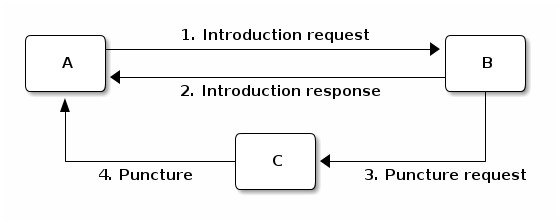
\includegraphics[width=.9\linewidth]{walk.png}
\caption{\label{fig:walk}Peer discovery mechanism}
\end{figure}

Our peer discovery mechanism illustrated in Figure~\ref{fig:walk}
consists of four phases:
\begin{description}
\item[{phase 1:}] peer A chooses a peer B from its neighbourhood and it
sends to peer B an introduction-request;
\item[{phase 2:}] peer B chooses a peer C from its neighbourhood and sends
peer A an introduction-response containing the address
of peer C;
\item[{phase 3:}] peer B sends to peer C a puncture-request containing the
address of peer A;
\item[{phase 4:}] peer C sends peer A a puncture message to puncture a
hole in its own NAT.
\end{description}

These four phases constitute \emph{a step}, and multiple steps constitute a
\emph{walk}.  By walking, each peer discovers a set of known peers which we
define as its \emph{neighbourhood}.

The remainder of this document explains the walker mechanism in detail
and gives the reasoning behind our design choices.  Section~\ref{sec-2} explains how we handle addresses and
identities using candidates, Section~\ref{sec-3} explains how peer
A chooses another peer from its neighbourhood, Section~\ref{sec-4} explains how peer B chooses another peer from its
neighbourhood, Section~\ref{sec-5} explains how peer B
determines peer A's LAN and WAN address, Section~\ref{sec-6}
explains how peer A determines its own WAN address, Section~\ref{sec-7} explains how the walker tries to follow the 5 second rule,
Section~\ref{sec-8} explains public key exchange, and
finally, Section~\ref{sec-9} explains what debug output to expect.
\section{IP addresses and member identities}
\label{sec-2}
In Dispersy, each peer needs to be able to verify the identities of
other peers because we use a right management mechanism.  According to
our right management mechanism, each peer has different access rights
based on the history of rights granted and revoked.  To this end, we
use public/private key pairs to allow peers to cryptographically
identify themselves.  The public/private key pair of a peer represents
a single Member instance which signs or verifies the messages created
by the peer itself or other peers, respectively.

Ideally, we want to assign one IP address to each member, and have
this mapping be the same for every peer in the system.  However, an IP
address may change between successive sessions or some peers may
assign the same IP address to a Member (i.e. someone behind a
symmetric NAT uses different ports for communication with other
peers).

For those reasons, besides a Member (i.e. the cryptographic key) we
use an additional instance, named a Candidate which is a temporary
pointer to the current IP address of the corresponding peer.

In order to provide a mapping between Members and Candidates, we
create for every Candidate a list of Member instances seen at this
address.  In other words, once having found a Member at a specific IP
address, we associate this member with the corresponding Candidate.
We note that this mapping is temporary,

\subsection{Candidate categories}
\label{sec-2-1}
Each Candidate maintains time stamps for important events taking place
during a walk, i.e. the last time of an introduction-request.  Using
these time stamps, we assign Candidates into four categories: \emph{walk},
\emph{stumble}, \emph{intro}, and \emph{none}.  These categories determine how we can
use Candidates during a walk.  Each Candidate is assigned only to one
category, and this category may change over time.

Below, we describe the four categories and the assignment process
using the example of peers A, B, and C from our illustration in
Figure~\ref{fig:walk}.  When communicating peers update several time
stamps that are used to compute how long ago an event occurred.

Peer A computes the \emph{walk difference} of peer B by taking the
difference between the current time and receiving an
introduction-response to an introduction-request from peer B.  Peer B
computes the \emph{stumble difference} of peer A by taking the difference
between the current time and receiving an introduction-request from
peer A.  Peer A computes the \emph{intro difference} of peer C by taking
the difference between the current time and receiving an
introduction-response introducing peer C.

Using the computed time differences a peer assigns all other peers in
one of the four categories:
\begin{description}
\item[{walk}] when its walk difference is less or equal to the \emph{walk
lifetime},
\item[{stumble}] when it is \emph{not} a walk-Candidate and its stuble
difference is less or equal to the \emph{stumble lifetime},
\item[{intro}] when it is neither a walk or a stumble-Candidate, and its
intro difference is less or equal to the \emph{intro lifetime},
and
\item[{none}] when it does not fulfil the criteria for its assignment to
one of the previously mentioned categories.
\end{description}

We set both the walk lifetime and the stumble lifetime equal to 57.5
seconds because most NAT boxes close a punctured ‘hole’ 60 seconds
after receiving the last packet.  Moreover, we set the intro lifetime
equal to 27.5 seconds because most NAT boxes close a punctured ‘hole’
after 30 seconds when no packets are received through
it\footnotemark[1]{}.
\subsection{(Un)verified candidates}
\label{sec-2-2}
The Dispersy code provides two main methods to obtain available
Candidate instances: the dispersy\_yield\_candidates
method\footnote{Implemented in the Community class, see dispersy/community.py} returns an iterator with all walk, stumble, and
intro-Candidate instances, in a randomised order.  Note that
intro-Candidates are \emph{unverified}, i.e. we have only heard about their
existence, but did not actually have any contact with them ourselves.

The dispersy\_yield\_verified\_candidates method\footnotemark[3]{} returns an
iterator with all walk and stumble-Candidate instances, in a
randomised order.  We call these Candidates \emph{verified} because we have
received a message from them at most 57.5 seconds ago (i.e. the walk
and stumble lifetime).

This means that, unless the peer went offline in the mean time, the
peer is still there and the NAT has, most likely, not closed yet.
Note that there are NATs that close within 57.5
seconds\footnotemark[1]{}, those will not be reachable.

Because of this, communicating with verified candidates is often
better than using unverified candidates.
\subsection{Candidates we can walk towards}
\label{sec-2-3}
A peer is only allowed to walk towards a Candidate when the Candidate
is eligible for a walk namely, it meets the two criteria described
below:
\begin{enumerate}
\item the category is either walk, stumble, or intro
\item the last time that this peer walked to this specific candidate,
occurred at least \emph{eligible delay} second ago.
\end{enumerate}

We have chosen 27.5 seconds for the eligible delay, with the exception
of bootstrap candidates which require a 57.5 seconds of eligible
delay.  As a result, the bootstrap peers are not contacted to
frequently.  This feature was initially introduced to reduce the
numbers of walks towards trackers in overlays with few peers.
\section{Who to walk to}
\label{sec-3}
In \textbf{phase 1} of the walk (as illustrated in Figure~\ref{fig:walk}), peer
A chooses a known peer B from its neighbourhood and sends it an
introduction-request.  The dispersy\_get\_walk\_candidate
method\footnotemark[3]{} chooses peer B and returns a Candidate instance
pointing to it.  If there are no available eligible candidates, this
method returns None.

The choice of a Candidate to walk determines the size of the
neighbourhood of peer A.  Based on its walks, peer A is able to know
at most 11 Candidates because according to our design, a peer takes
one step every 5 seconds (see Section~\ref{sec-7}).  As a result
in a walk lifetime window of 57.5 seconds, it can take at most 11
steps.  Nevertheless, other peers may chose to walk to peer A.  Hence,
the incoming walks to peer A, that occurred within the stumble
lifetime window, increase the size of its neighbourhood accordingly.

Assuming that there is at least one eligible Candidate in every
category, the selection strategy can be simplified in the following
rules.  Peer A chooses with probability:
\begin{itemize}
\item 49.75\% to revisit the \emph{oldest} eligible walk-Candidate,
\item 24.825\% to visit the \emph{oldest} eligible stumble-Candidate,
\item 24.825\% to visit the \emph{oldest} eligible intro-Candidate, and
\item 0.5\% to visit a \emph{random} eligible Candidate from the predefined list
of bootstrap candidates.
\end{itemize}

If one category is empty, the probabilities of choosing a peer from
this category becomes 0.  In Table~\ref{tbl:who-to-walk-towards}, we present
the probability of choosing categories when some of these categories
are empty.  The first column \emph{has-WSIB} shows in binary form if there
is at least one walk, stumble, intro, or bootstrap candidate available
by setting the corresponding bit equal to 1.  For example, 1000 means
that the only available candidates are walk candidates.

\begin{table}[htb]
\caption{\label{tbl:who-to-walk-towards}Chance to select a category based depending on which categories has eligible candidates.}
\centering
\begin{tabular}{r|rrrrr}
has- &  &  &  &  & \\
WSIB & walk & stumble & intro & boot & none\\
\hline
0000 &  &  &  &  & 100\%\\
0001 &  &  &  & 100\% & \\
0010 &  &  & 100\% &  & \\
0011 &  &  & 99.5\% & 0.5\% & \\
0100 &  & 100\% &  &  & \\
0101 &  & 99.5\% &  & 0.5\% & \\
0110 &  & 50\% & 50\% &  & \\
0111 &  & 49.75\% & 49.75\% & 0.5\% & \\
1000 & 100\% &  &  &  & \\
1001 & 99.5\% &  &  & 0.5\% & \\
1010 & 50\% &  & 50\% &  & \\
1011 & 49.75\% &  & 49.75\% & 0.5\% & \\
1100 & 50\% & 50\% &  &  & \\
1101 & 49.75\% & 49.75\% &  & 0.5\% & \\
1111 & 49.75\% & 24.825\% & 24.825\% & 0.5\% & \\
\end{tabular}
\end{table}

Malicious peers can easily pollute our neighbourhood by walking
towards a peer from multiple distinct addresses and adding an
arbitrary number of stumble-Candidates to its neighbourhood.  To avoid
such a neighbourhood pollution, we assume that a successfully visited
peer is safe.  Hence, half of the time we revisit such a peer
(i.e. from the walk category) while the remaining 50\% is evenly spread
between the intro category and the risky stumble category.  Method
dispersy\_get\_walk\_candidate implements this design.

\subsection{Dissemination experiments}
\label{sec-3-1}
During experiments that want to focus on dissemination speed, it is
possible to only visit bootstrap-Candidates during the bootstrap
process.  Otherwise there is a 0.5\% chance each step to visit a
bootstrap peer and not get any new data (since the bootstrap peers do
not participate in data dissemination).

Approximately 450 bootstrap peers\footnote{one peer takes 12 steps per
minute, 500 peers take 90,000 steps in 15 minutes, 0.5\% will be
towards bootstrap peers, i.e. 450 steps.} will be unnecessarily
visited in a 15 minute experiment where 500 peers disseminate data.
When this is undesirable, perhaps because you do not want to explain
why certain steps do not yield any new data, the file
minimal\_bootstrap.diff will remove the 0.5\% chance to visit a
bootstrap peer.  This will result in the combinations shown in
Table~\ref{tbl:suggested-who-to-walk-towards}.

\begin{table}[htb]
\caption{\label{tbl:suggested-who-to-walk-towards}Suggested chance to select a category based depending on which categories has eligible candidates.}
\centering
\begin{tabular}{r|rrrrr}
has- &  &  &  &  & \\
WSIB & walk & stumble & intro & boot & none\\
\hline
0000 &  &  &  &  & 100\%\\
0001 &  &  &  & 100\% & \\
0010 &  &  & 100\% &  & \\
0011 &  &  & 100\% &  & \\
0100 &  & 100\% &  &  & \\
0101 &  & 100\% &  &  & \\
0110 &  & 50\% & 50\% &  & \\
0111 &  & 50\% & 50\% &  & \\
1000 & 100\% &  &  &  & \\
1001 & 100\% &  &  &  & \\
1010 & 50\% &  & 50\% &  & \\
1011 & 50\% &  & 50\% &  & \\
1100 & 50\% & 50\% &  &  & \\
1101 & 50\% & 50\% &  &  & \\
1111 & 50\% & 25\% & 25\% &  & \\
\end{tabular}
\end{table}
\section{Who to introduce}
\label{sec-4}
In \textbf{phase 2} of the walk, peer B chooses a known peer C from its
neighbourhood and introduces it to peer A.  The
dispersy\_get\_introduce\_candidate method\footnotemark[3]{} chooses peer C
from the verified available candidates and returns it, or, when no
candidates are available, it returns None.

Using dispersy\_get\_introduce\_candidate returns a verified candidate in
semi round \emph{robin fashion}.  To this end each Community maintains two
dynamic iterators\footnotemark[3]{} \_walked\_candidates and
\_stumbled\_candidates which iterate over all walk-Candidates and
stumble-Candidates in round-robin, respectively.

\begin{figure}{}
\centering
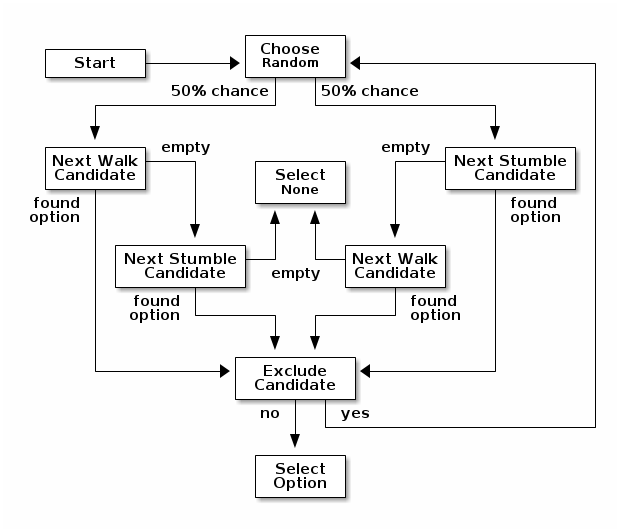
\includegraphics[width=.9\linewidth]{who-to-introduce.png}
\caption{\label{fig:who-to-introduce}Introduction peer selection mechanism}
\end{figure}

In Figure~\ref{fig:who-to-introduce}, we present the selection process
of a Candidate.  In most cases, this process is simplified in the
following steps:
\begin{enumerate}
\item choose either the walk-Candidate or stumble-Candidate iterator,
\item select the next Candidate in the iterator if it is not excluded,
otherwise go back to step 1.
\end{enumerate}

\subsection{Candidate exclusion}
\label{sec-4-1}
Peer B can not introduce peer C to A when:
\begin{itemize}
\item C and A are the same Candidate,
\item C and A are both behind a NAT and they are not within the same LAN,
\item C is behind a tunnel while A is not behind a tunnel.  Peer C is
behind a tunnel when all messages it sends have a \texttt{FFFFFFFF} prefix.
In this case, it can only receive messages with this prefix.
Tunnelling has been introduced to Dispersy at the end of 2012 so
that traffic is send through libswift.  Dispersy recognises the
\texttt{FFFFFFFF} prefix without using libswift.  However, older Dispersy
clients cannot recognise this prefix and they see it as a part of
the message.  Since older and newer versions of Dispersy are not
distinguishable, we are currently considering all peers to use an
older version of Dispersy.
\end{itemize}
\subsection{Duplicate candidates}
\label{sec-4-2}
It is possible that peer B introduces an already known peer to peer A.
We could have excluded the known peers by having peer A sending a list
of known peers that peer B can exclude.  However, we decided not to do
this because:
\begin{enumerate}
\item it would increase the size of the introduction-request,
\item it would give peer B information about peer A,
\item the larger the overlay, the smaller the chance that peer B will
introduce a peer that peer A already knows.
\end{enumerate}
\section{LAN and WAN address}
\label{sec-5}
In \textbf{phase 2} of the walk, peer B determines the LAN and WAN address of
peer A by using the UDP header (i.e. the sock\_addr) of the incoming
introduction-request combined with the WAN and LAN address as reported
by A, as it is illustrated by Figure~\ref{fig:determine-lan-wan}.

\begin{figure}{}
\centering
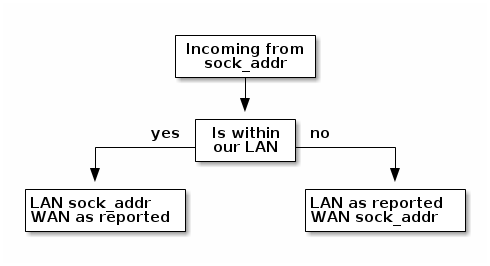
\includegraphics[width=.9\linewidth]{determine-lan-wan.png}
\caption{\label{fig:determine-lan-wan}Determine the LAN or WAN address of a peer}
\end{figure}

We implement this in method estimate\_lan\_and\_wan\_addresses using a
simple rule: when peer B sees that the corresponding message
originates from its LAN, it decides that peer A’s LAN address is the
sock\_addr.  If the message originates outside its LAN, then peer A’s
WAN address is the sock\_addr[fn::The word 'estimate' is for historical
reasons since this code was not able to make this decision as cleanly
as is described here.].

Dispersy determines whether an address originates within its own LAN
or not by checking if it corresponds with one of its local interfaces,
with regards to its netmask.  We do this using the
\_get\_interface\_addresses method\footnote{Implemented in the Dispersy class, see dispersy/dispersy.py} and the Interface
instances that it returns.

Peer B uses the result of this estimation to update the lan\_address
and wan\_address properties\footnote{Implemented in the WalkCandidate class, see dispersy/candidate.py} of the Candidate instance
pointing to peer A.  These values are also added to the
introduction-response, allowing peer A to assess its own WAN address,
as discusses in Section~\ref{sec-6}.
\section{WAN address voting}
\label{sec-6}
In \textbf{phase 2} of the walk, peer A receives an introduction-response
containing the LAN and WAN address that peer B believes it has.  This
\emph{dial back} allows peer A to determine how other peers perceive it,
and thereby whether a NAT is affecting its address.

When peer A is not affected by a NAT the voting will provide it with
its own address.  This is useful when peer A and B are both within the
same LAN while peer C is not.  In this case peer A will send an
introduction-request (which includes the WAN address determined by
voting) to peer B, peer B will inform peer C of both A’s LAN (as
determined by the UDP header) and WAN address (as reported by A),
allowing peer C to determine that peer A is not within its LAN
address, hence it will use peer A’s reported WAN address to puncture
its own NAT.

When a NAT affects peer A the voting will provide information about
the type of NAT, i.e. the connection type, that it is behind, as
described below.  This connection type effects who a peer introduces
when receiving an introduction-request, see Section~\ref{sec-4}.

Most of the magic happens in the wan\_address\_vote method\footnotemark[5]{}
and goes roughly as follows:
\begin{enumerate}
\item remove whatever B voted for before,
\item if the address is valid and B is outside our LAN then add the vote
\item select the new address as our WAN address if it has equal or more
votes than our current WAN address.  Note that changing our WAN
address also makes us re-evaluate our LAN address;
\item determine our connection type based on the following rules:
\begin{description}
\item[{public}] when all votes have been for the same address and our
LAN and WAN addresses are the same,
\item[{symmetric-NAT}] when we have votes for more than one different
addresses, and
\item[{unknown}] in all other cases.
\end{description}
\end{enumerate}

\subsection{Cleanup old voting data}
\label{sec-6-1}
To allow for changes in the connectivity, i.e. when running on a
roaming machine that changes IP addresses periodically, we must remove
older votes, by calling the wan\_address\_unvote method\footnotemark[5]{},
that may no longer apply.

Dispersy does this by periodically \emph{(every five minutes)} checking for
obsolete Candidate instances.  Where we consider a Candidate to be
obsolete when the last walk, stumble, or intro was more than
\emph{lifetime} seconds ago, where lifetime is three minutes.  This means
that it can take anywhere between five and eight minutes before
removing old votes.
\section{The 5 second rule}
\label{sec-7}
When we decided on the design of the walker we took into account the
following factors:
\begin{enumerate}
\item a significant number of NAT devices close a port 60 seconds after
receiving the last packet though it\footnote{Do not confuse with NAT
   devices closing a port 30 seconds after puncturing it without
   receiving any packets through it}, and
\item taking a step involves performing the bloom filter synchronisation.
Synchronisation is not described in this report.
\end{enumerate}

Obviously when we take more steps the neighbourhood will contain more
walk and intro-Candidates (and since other peers also take more steps
the neighbourhood will also, on average, contain more
stumble-Candidates).  This would advocate taking as many steps as
possible.

However, every step also has a cost associated to it, the majority
being in the bloom filter synchronisation.  At the time we wanted
every step to perform a synchronisation, and given that some peers
might receive multiple incoming steps around the same time, we decided
on a reserved value of 5 seconds.  We expect this to be sufficient to
perform one synchronisation for ourselves and, in the worst case,
multiple incoming synchronisations.

Nowadays we have introduced mechanisms to reduce the workload by not
always performing a bloom filter synchronisation, hence the 5 second
rule is not strictly necessary anymore, however, the code contains
constants derived from 5 seconds, making it difficult to change (see
\ref{sec-7-3}).

\subsection{Walking in a single overlay}
\label{sec-7-1}
In the worst case, creating a bloom filter is one of the most CPU
intensive parts of Dispersy.  Below, we present an example of a naive
approach where we simply schedule 5 seconds between each step.  For
simplicity, we will assume that it takes 1 second to create a bloom
filter.

The schematic below shows a time line with \emph{+} every 5 seconds when a
step should take place.  It shows that creating the bloom filter is
causing walker \emph{X} to take a step once every 6 seconds instead of
every 5 seconds.  Furthermore, a large delay caused by task T
increases the gap between steps even further, resulting in only 7
steps instead of 10 which is the expected number of steps.

\begin{verbatim}
                delayed steps
+----+----+----+----+----+----+----+----+----+  (time line)
            TT            TT            TT      (task T)
X     X       X     X       X     X       X     (steps overlay X)
\end{verbatim}
\subsection{Walking in multiple overlays}
\label{sec-7-2}
The previous naive approach causes the gap between walks to be larger
than the intended 5 seconds, this in turn results in fewer walks,
hence slower data dissemination and fewer available candidates.  The
gap between walks will only get larger when we need to maintain
multiple overlays at the same time.  In this case the naive approach
would result in both overlays \emph{X} and \emph{Y} walking immediately after
one another, causing a spike in CPU traffic, as seen in the schematic
below.

\begin{verbatim}
     delayed steps with multiple overlays
+----+----+----+----+----+----+----+----+----+  (time line)
            TT            TT            TT      (task T)
X     X       X     X       X     X       X     (steps overlay X)
   Y     Y     Y     Y       Y     Y       Y    (steps overlay Y)
\end{verbatim}

We address both of these problems by what we call a \emph{self healing
walker}, implemented in the \_candidate\_walker method\footnotemark[5]{}.
This walker takes into account both the number of overlays and the
time between walks in individual overlays.  The self healing walker
has two major features:
\begin{itemize}
\item predicting the time when the next walk should occur to remove the
delays the naive approach would introduce
\item allowing more than one step in a single overlay within 5 seconds, as
seen in the schematic below where the lowercase \emph{x} and \emph{y} are
within 5 seconds of the previous step taken in its overlay.
\end{itemize}

\begin{verbatim}
              self healing walker
+----+----+----+----+----+----+----+----+----+  (time line)
          TT             TT             TT      (task T)
X    X      X  x    X      X  x    X      X  x  (steps overlay X)
   Y     Y    Y   y    Y     Y   y    Y     Y   (steps overlay Y)
\end{verbatim}

To preserve resources, Dispersy will tell a community not to perform a
bloom filter synchronisation (while still performing the walk to
maintain the neighbourhood) when the previous step was less than 4.5
seconds ago.  Since this will usually occur under heavy CPU load, the
benefit is that it will reduce the load since synchronisation is the
most expensive part of taking a step.

When we detect that the previous walk in an overlay was more than 5
seconds ago, a \emph{walk reset} will occur to ensure we do not walk to
often.  This is especially useful when a computer running Dispersy
goes into sleep mode, when it wakes up the walk may be hours behind,
the walk reset will ensure that Dispersy doesn’t try to catch up with
the sleeping time by taking thousands of steps.
\subsection{Walk multiplier}
\label{sec-7-3}
Sometimes it can be useful to change the 5 seconds delay between steps
into something else.  The problem is that all derived values must be
appropriately changed.  The best way to do this is to multiply all
these values with the same constant.

The file walk\_multiplier.diff will modify all these constants (as
known at October 2013).  Changing the \texttt{WALK\_MULTIPLIER}
constant\footnote{Implemented in the WalkCandidate class, see dispersy/candidate.py} to 2 will result in a step every 10.0 seconds,
i.e. slowing down the walker.  Conversely, changing the constant to
0.5 will result in a step every 2.5 seconds, i.e. speeding up the
walker.
\section{Transferring the public key}
\label{sec-8}
The signed walker messages introduction-request and
introduction-response used in Section~\ref{sec-1} do not contain the
public key of the signer, we transfer this key using a
missing-identity request and a identity message response.

Luckily this is only needed for public keys that we do not yet have,
hence the first time that we encounter a peer the walk actually
follows Figure~\ref{fig:walk-identity}.

\begin{figure}{}
\centering
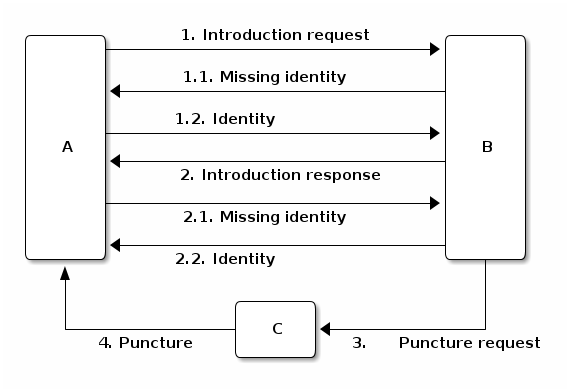
\includegraphics[width=.9\linewidth]{walk-identity.png}
\caption{\label{fig:walk-identity}Peer dispersy mechanism between unknown peers}
\end{figure}
\section{Debug output}
\label{sec-9}
Dispersy uses the standard Python logger to output different message
levels, i.e. DEBUG, INFO, WARNING, and ERROR.  When enabling DEBUG
messages the logger in dispersy/endpoint.py will log all incoming and
outgoing packets, including their name when possible.  This can give
valuable information when something does not follow the expected
behavior.

\subsection{Bootstrapping}
\label{sec-9-1}
To bootstrap an overlay, each node contacts one of the bootstrap
servers.  If nodes have never encountered this bootstrap server
before, they need to exchange public keys.  This results in the
following DEBUG output:

\begin{verbatim}
 dispersy-introduction-request -> 130.161.211.245:6422   132 bytes
     dispersy-missing-identity <- 130.161.211.245:6422    51 bytes
             dispersy-identity -> 130.161.211.245:6422   177 bytes
dispersy-introduction-response <- 130.161.211.245:6422   126 bytes
     dispersy-missing-identity -> 130.161.211.245:6422    51 bytes
             dispersy-identity <- 130.161.211.245:6422   141 bytes
\end{verbatim}
\subsection{Building a neighbourhood}
\label{sec-9-2}
After have walked for some steps, each node builds its neighbourhood.
Below we see that we contact someone at 74.96.92.***:7759.  Nodes no
longer need to exchange public keys, but only the incoming puncture
message from 84.209.251.***:7759 is from someone not yet encountered,
hence we exchange identities immediately.

\begin{verbatim}
 dispersy-introduction-request ->    74.96.92.***:7759   132 bytes
dispersy-introduction-response <-    74.96.92.***:7759   144 bytes
             dispersy-puncture <-  84.209.251.***:7759   125 bytes
     dispersy-missing-identity ->  84.209.251.***:7759    51 bytes
             dispersy-identity <-  84.209.251.***:7759   177 bytes
\end{verbatim}
\subsection{Candidate statistics}
\label{sec-9-3}
Dispersy provides a logger with the name
dispersy-stats-detailed-candidates.  When enabling DEBUG level
messages for this logger, it will output a summary of its
neighbourhood every five seconds.  The example below is the summary as
seen shortly after contacting 74.96.92.***:7759, see below:

\begin{verbatim}
--- 8164f55c2f828738fa779570e4605a81fec95c9d Community ---
  4.7s  E  intro   unknown       {192.168.1.35:7759 84.209.251.***:7759}
  9.7s  E  intro   unknown       {192.168.25.100:7759 177.157.54.***:7759}
 14.8s  E  intro   unknown       {192.168.0.3:34728 188.242.194.***:34728}
 19.9s  E  intro   unknown       {192.168.3.101:7759 67.33.160.***:7759}
 24.4s  E  intro   unknown       {192.168.178.21:7759 188.154.8.***:7759}
  5.0s     walk    unknown       {192.168.1.18:7759 74.96.92.***:7759}
 10.0s     walk    unknown       {192.168.0.100:7761 84.251.49.***:7761}
 15.0s     walk    symmetric-NAT {178.164.145.6:7759 94.21.97.***:7759}
 20.0s     walk    unknown       {192.168.1.27:7759 87.18.61.***:16409}
 25.0s     walk    symmetric-NAT {90.165.123.***:7759}
 30.0s  E  walk    unknown       {192.168.1.172:7759 76.115.137.***:7759}
 35.0s  E  walk    unknown       {192.168.2.3:7759 97.91.131.***:7759}
 45.0s  E  walk    unknown       {192.168.1.51:7749 109.208.189.***:7749}
 50.0s  E  walk    unknown       {192.168.0.3:7759 180.145.124.***:7759}
 55.0s  E  walk    unknown       {192.168.0.2:7759 83.153.18.***:7759}
\end{verbatim}

The summary shows that the Candidate at 74.96.92.***:7759 is currently
a walk-Candidate with age 5.0 seconds, i.e. we sent the
introduction-request 5.0 seconds ago.

Furthermore, there is an intro-Candidate at 84.209.251.***:7759, which
is the introduced Candidate from when we received a response to this
walk 4.7 seconds ago.  Note that this Candidate has the character \emph{E}
which signifies that this Candidate is eligible for a walk.

%% \section{Conclusion}
%% This technical report shows how the default Dispersy implementation
%% handles peer discovery.  It also shows what can be modified to achieve
%% different behaviour.

\bibliographystyle{ieeetr}
\bibliography{PDS-2013-009}

% Emacs 24.2.1 (Org mode 8.2.3c)
\end{document}
